%%%%%%%%%%%%%%%%%%%%%%%%%%%%%%%%%%%%%%%%%%%%%%%%%%%%%%%%%%%%%

\mainmatter
\setcounter{page}{1}

\lectureseries[\course]{\course}

\auth[\lecAuth]{Lecturer: \lecAuth\\ Scribe: \scribe}
\date{November 5, 2009}

\setaddress

% the following hack starts the lecture numbering at 21
\setcounter{lecture}{20}
\setcounter{chapter}{20}

\lecture{Midterm Notes}

\section{Material Covered}
The midterm exam is an open-book and open-notes test to verify that each student individually understands the basic concepts of the course (so far). The midterm will cover all the handouts and all the material (Chap.1, Chap. 2, Chap. 3,  Section 4.1, Section 4.2, Chap. 6, Section 7.3, Section 7.5, Section 7.6, Section 10.1 in the text book) taught during the lectures up to and including Tuesday November 3, 2009.

\section{2006-2d/2007-1d}
For the unweighted parameter estimate $\hat{\theta}_N$ is given by
$$\hat{\theta}_N = \left[\frac{1}{N}\sum_{t=1}^N\vp(t)\vp^T(t)\right]^{-1}\left[\frac{1}{N}\sum_{t=1}^N\vp(t)y(t)\right]$$
To prove that the cross-correlation function $\hat{R}_{\epsilon u}^N(\tau)$ between prediction error $\epsilon(t,\hat{\theta}_N)$ and input $u(t)$ satisfies $\hat{R}_{\epsilon u}^N(\tau)=0$ for $\tau=0,1,\ldots,n$ we have to know that
\begin{itemize}
\item $u\perp e$
\item $E\{e(t)u(t-\tau)\}=0$
\item $\lim_{N\to\infty}\hat{R}_{eu}^N(\tau))=0$. This one we can never compute.
\end{itemize}
All of those items are equivalent. Suppose we get ``white noise'' inputs and error in \textsc{Matlab} using \texttt{e=randn(N,1)} and \texttt{u=randn(N,1)}. Is $\hat{R}_{eu}(\tau)=0 ~\forall \tau$? Not in \textsc{Matlab} because the randomness is finite. At some point the random sequence will begin to repeat.

However, notice that the LS estimate gives the prediction error as $\epsilon(t)=y(t)-\vp^T(t)\hat{\theta}_{LS}^N$. This means that $\hat{R}_{\epsilon u}^N(\tau)=0$ for $\tau=1,\ldots,n$, where $n$ is the number of past inputs in $\vp(t)$. This is true because of the way the LS estimate is constructed as an orthogonal projection of the output $y(t)$ onto the space of $\vp^T(t)\theta$ while letting $\theta$ vary. See Figure \ref{fig:mt062d2}. This guarantees that $\epsilon(t)$ is orthogonal to $\vp^T(t)$ which contains the past inputs and outputs. Since the prediction error is orthogonal to the past ($n$) inputs the cross-correlation is zero. See Figure \ref{fig:mt062d1}.

\begin{figure}[ht!]
  \centering
  \includegraphics[width=.5\textwidth]{images/mt062d2}
  \caption{Projection of output $y(t)$ onto space of $\vp^T(t)\theta$ with $\theta$ varying. Shows projection error.}
  \label{fig:mt062d2}
\end{figure}

\begin{figure}[ht!]
  \centering
  \includegraphics[width=.5\textwidth]{images/mt062d1}
  \caption{Cross-correlation function between noise error and input, prediction error and input.}
  \label{fig:mt062d1}
\end{figure}

We can also see this from the equation
$$\sum\vp(t)y(t) = \sum\vp(t)\vp^T(t)\underbrace{\theta}_{LS} + \underbrace{\sum\vp(t)\epsilon(t)}_{=0, \vp\perp\epsilon}$$

\section{2006-2e/2007-1e}
As long as $\{u(t)\}$ is white and
$$G_0(q)=\frac{B_0(q)}{A_0(q)}$$
then
$$\lim_{N\to\infty}\thn(k)=g_0(k)$$
To show that this happens look at \S\ref{sec:peconsistency}. The parameter $\theta$ contains the impulse response coefficients so this estimate would go to $g_0(k)$. Remember that we must be looking at an FIR model where the noise filter is
$$H_0(q)=\frac{1}{A(q)}$$
See \S\ref{sec:carefulwhitenoise} for more details on how the filter will cause the measured noise, $v(t)$, to be colored even if the actual noise, $e(t)$, is white for any other model than FIR. If the noise is colored then the terms in the lower block matrix of $R_{\vp v}(0)$ will not zero.

\section{2007-1c}
This is just getting $\thn=R^{-1}(N)f(N)$ where $R(N)$ and $f(N)$ are made up of elements of $R_{yu}(\tau)$ and $R_u(\tau)$. See \S\ref{sec:lsecovfns} for more details.

\section{2006-1b}
Notice that
\begin{align*}
R_u(\tau) &= \sin(\w t)\sin(\w t-\tau) \\
R_u(0) &= \sin^2(\w t) \\
R_u(1) &= \sin(\w t)\sin(\w t-1) \\
R_u(2) &= \sin(\w t)\sin(\w t-2)
\end{align*}
Plug those into the $\mathbf{R}$ matrix. It is easy to see that $R_u(0)$ and $R_u(1)$ are independent and form the first $2\times 2$ block of $\mathbf{R}$, therefore $\text{rank}(\mathbf{R})=2$. To see if the rank is any greater we can plug in $R_u(2)$. However, it is easy to see that $R_u(2)$ can be formed as a linear combination of $R_u(1)$ and still results in $\text{rank}(\mathbf{R})=2$. By induction, $\{u(t)\}$ is persistently exciting of order $2$.

%%%%%%%%%%%%%%%%%%%%%%%%%%%%%%%%%%%%%%%%%%%%%%%%%%%%%%%%%%%%%